
\let\textcircled=\pgftextcircled
\chapter{Modelling the effect of actuator-like behavior in dielectric elastomer generators}
\label{chap:1}

\initial{T}his chapter is based on the paper ''Self-stabilizing Dielectric Elastomer Generators``, published in the edition number 3 from Volume 26 of Smart Materials and Structures in 2015.

Despite many advantageous characteristics of DEG, there are still issues to overcome, including the need for charging at every cycle to produce an electrical output. Self-priming Circuits (SPCs) are one possible solution, storing part of the electric energy output of one cycle to supply as input for the next, producing a voltage boost effect. Until now, studies regarding SPCs neglect to consider how the increasing voltage will create an electromechanical response and affect the DEG when driven by an oscillatory mechanical load. In the present work we model this force-based actuation, including coupling between the DEG and SPC, in order to predict the dynamics of the system. In such cases, the DEG has a mechanical response when charged (actuator behaviour), and as the voltage increases, this actuation-like effect increases the capacitance values that bound the cycle. We show how this inherent nonlinearity yields a reduction in the DEG’s capacitance swing and reduces the performance of the SPC, but also self-stabilizes the system.  This stability is useful in the design of robust DEG energy harvesters that can operate near to, but not enter, failure mode.



%=======

\section{Introduction}
\label{sec:intro}

Dielectric elastomers (DEs) are smart materials which can transduce mechanical into electrical energy and vice-versa, and as such have been exploited as actuators, sensors and for energy harvesting [1-7]. They consist of an elastic membrane coated with stretchable electrodes, together composing a flexible capacitor [8]. Once electrically charged, electrostatic forces acting normal (attractive) and parallel (repulsive) to the membrane are induced and deform it, yielding an actuator or “artificial muscle”. This electromechanical process can be also inverted; by cyclic stretching and relaxing with appropriately-timed charging, mechanical energy can be converted into electrical energy [6]. There are several possibilities for such a Dielectric Elastomer Generator (DEG) cycle, but their main characteristic is the conversion of stored strain energy into electrical energy, by allowing the material to relax once it is charged. This pushes like charges together and pulls opposing charges apart as the material goes from a thin and stretched, to a thicker and more relaxed, state. 
DEGs have been a focus of research effort, because they are able to harvest mechanical energy whilst also being cheap, lightweight, shock and corrosion insensitive, and having high energy density [6, 9, 10]. Although still unable to match the efficiency of other more established devices, such as electromagnetic generators [11-15], the characteristics of DEGs make them a promising technology to harvest energy from less explored energy sources, such as waves, or even to scavenge energy from human body motion [16-20]. 
It has been shown that, during a force-based cycle, when the DEG is stretched due to a forcing or pressure oscillation without mechanical stretch limitations, there is an actuation-like effect after the charging phase [21]. This actuation is the same as for conventional Dielectric Elastomer Actuators, where the induced Maxwell stress due to charge separation causes mechanical deformation [7]. It is expected that the higher the voltage used in the charging phase, the higher is the resulting stretch due to the actuation effect. Since electrical energy output, and consequently net energy gain, is proportional to the electrical energy input [22], it is important to study the best methods for charging, and their consequences.

\begin{figure}[ht]
\begin{center}
\begin{tabular}{c}
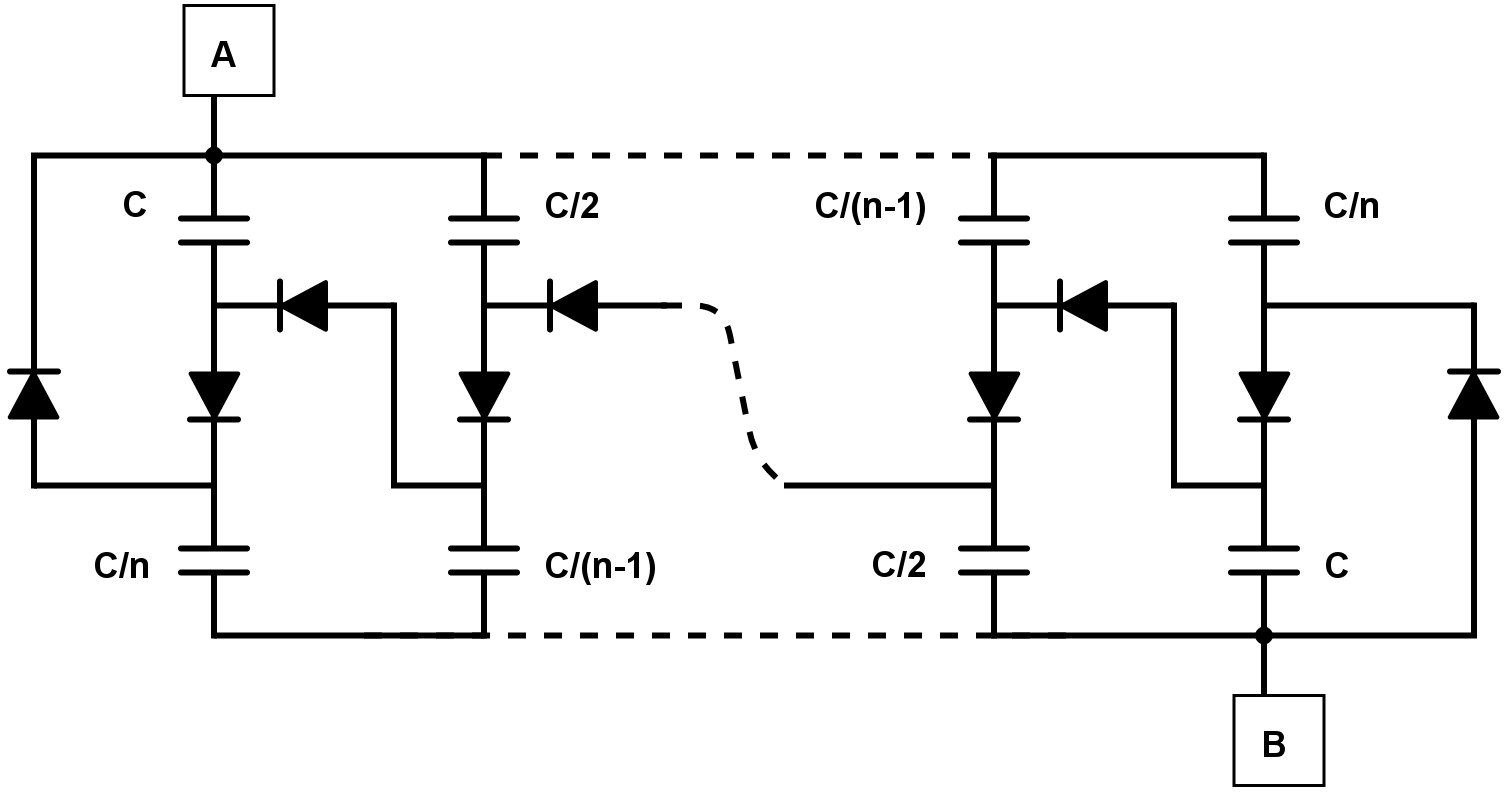
\includegraphics[height=6cm]{fig04/SPC_general.png}
\end{tabular}
\end{center}
\caption 
{ \label{fig:SPC_general}
Self-Priming circuit general scheme. $C$ is the maximum capacitance in the circuit, while $n$ is the number of stages of the circuit.}
\end{figure}  

Focusing on this charging phase of the DEG cycle, self-priming circuits (SPCs) [10] are one of the most attractive approaches for electrically charging a DEG. Self-priming circuits are able to store part of the energy output from a cycle and supply it as input for the following cycle. They consist of an arrangement of diodes and capacitors, as shown in figure 1. Since DEGs behave as a voltage booster mechanism if operated open-circuit during the relaxing phase [22], SPCs are able to start the energy harvesting process from low voltages and boost it until higher voltages are achieved. Since the energy generated per cycle depends on the voltage primed during the charging phase [22], SPCs allow us to use DEGs in conditions when managing the high voltage charging and discharging at each cycle is not an option. In such scenarios, once primed by a small initial charge, DEG-SPC systems have a passive boost effect and increased energy output. Figure 2 shows how the boost occurs in DEG-SPC systems during a cycle. From a charged and stretched state, the DEG relaxes (phase 1) and its voltage increases until it reaches the threshold to discharge into the SPC. Charges are then transferred to the SPC (phase 2) until the minimum stretch level of the cycle is achieved. As the DEG starts to stretch (phase 3), its voltage starts to decrease, until it reaches the threshold to receive charge from the SPC (phase 4).

\begin{figure}[ht]
\begin{center}
\begin{tabular}{c}
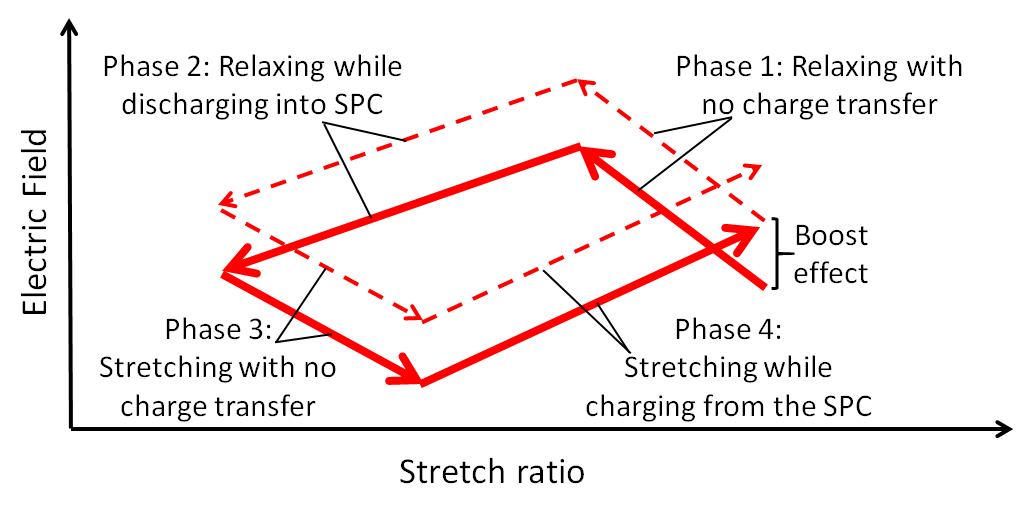
\includegraphics[height=6cm]{fig04/SPC_cycle_ph2.png}
\end{tabular}
\end{center}
\caption 
{ \label{fig:SPC_cycle}
Boosting cycle scheme in a DEG-SPC system.}
\end{figure}   


Several studies have been conducted on SPCs, from proposed design rules [24], to different layouts inverting parallel-series capacitors for charging and discharging of DEGs [25, 26]. Nevertheless, all these consider the DEG to be merely a variable capacitor attached to the SPC, cycling it in a position-based manner [27], between a low (relaxed) and a high (stretched) capacitance state.
In this paper, we investigate the behaviour of the DEG-SPC system in a force-based cycling scenario [27], a more realistic model of many real-world applications. As such, we are able to verify how the actuation-like behaviour of the DEG interferes with the boosting effect of the SPC. To do so, we start from a quasi-static analytical model and compare with simulations of an integrated fully dynamic numerical model. We also evaluate, using the numerical model, the trends in the frequency response analysis of the observed behaviour.
	Methods
We use an analytical mathematical model (described fully in [23]) to represent the behaviour of an ideal DEG-SPC system without electric load attached: the energy harvested in one cycle is completely used to prime the following one. In that scenario, we can describe the voltage gain in a single cycle, B, as [23]
\begin{equation}
B=\frac{C^2+(C_{\text{DEG}_\text{max}} + C_{\text{DEG}_\text{min}})C+C_{\text{DEG}_\text{max}}C_{\text{DEG}_\text{min}}}{C^2+(C_{\text{DEG}_\text{max}}/\omega^2 +C_{\text{DEG}_\text{min}}\omega^2)C+C_{\text{DEG}_\text{max}}C_{\text{DEG}_\text{min}}} 
\end{equation}
where 
\begin{equation}
\omega^2=  \frac{n+1}{n}
\end{equation}

$n$ and $C$ are the design parameters of the SPC (as shown in figure \ref{fig:SPC_general}), and $C_{\text{DEG}_\text{max}}$ and $C_{\text{DEG}_\text{min}}$ are, respectively, the maximum and minimum capacitances the DEG reaches in that cycle. Note that the DEG capacitance can be related to its physical dimensions as

\begin{equation}
C=\frac{e_r e_0 Vol}{z^2}
\end{equation}

where $e_r$ is the material relative permittivity, $e_0$ is the vacuum dielectric permittivity, $Vol$ is the (constant) total volume and $z$ the membrane thickness.
From \ref{eq:1}, we are also able to obtain the condition for the boost to exist, given by 
\begin{equation}
C_{\text{DEG}_\text{max}}>\omega^2 C_{\text{DEG}_\text{min}}
\end{equation}
Analysing the expected behaviour of a DEG-SPC system, we know – in contrast to conventional actuator behaviour – that maximum electric field will occur during the minimum stretch in a cycle [21]. Thus, we hypothesise an increased effect of the actuation in the minimum stretch position rather than in the maximum, and so the capacitance swing, $C_{\text{DEG}_\text{max}}/C_{\text{DEG}_\text{min}}$, will change cycle-by-cycle, since we expect $C_{\text{DEG}_\text{min}}$ to increase more than $C_{\text{DEG}_\text{max}}$. Considering a system with a fixed number of stages, $n$, if the capacitance swing is reduced, it will certainly affect the boost and will ultimately limit it. In this case, we have that, in the limit,
\begin{equation}
C_{\text{DEG}_\text{max}}/C_{\text{DEG}_\text{min}}= \omega^2
\end{equation}

leading to 
\begin{equation}
\lambda^+/\lambda^- =f(\omega)
\end{equation}

where $\lambda^-$ and $\lambda^+$ are, respectively, the minimum and maximum stretch ratios the material experiences in the cycle. The function $f$ will depend on the geometry and type of stretch to which the material is subjected to (pure-shear, equibiaxial, etc.).
Inserting (5) into the SPC model [23] leads to the relation between maximum ($V^+$) and minimum voltage ($V^-$) oscillation,

\begin{equation}
V^+/V^- = \omega^2
\end{equation}

Considering the scenario where the movement is bounded by the maximum force, $F^+$, and minimum force, $F^-$, we look for a stable periodic solution where there is no voltage boost between cycles, due to the change in the capacitance swing given by the increase in voltage levels. To do so, we use the relation between force, $F$, stretch ratio, $\lambda$, and voltage, $V$, described by the function $F= h(\lambda,V)$, dependent on the electromechanical model chosen. At the known boundaries of minimum and maximum force, this gives
\begin{align}
F^-&=  h(\lambda^-,V^+)\\
F^+&=  h(\lambda^+,V^-) 
\end{align}

which together with (5) and (6) gives a closed system for $\lambda^-$, $\lambda^+$, $V^-$ and $V^+$. Although this requires a numerical solver for most realistic examples, we are able to provide an analytical solution for a small set of cases. For example, considering a Neo-Hookean model in pure shear conditions with quasi-static forcing (hence neglecting dynamic effects), we can write [21]
\begin{equation}
F_x=   \frac{Vol}{x_0}\left(G-e_r e_0 \left(\frac{V}{z_0} \right)^2 \right) \lambda_x-\frac{Vol G}{x_0 \lambda_x^3 }
\end{equation}

where $F_x$ is the applied force, $G$ is the shear modulus, $\lambda_x$   is the stretch ratio in the forcing direction, $e_r$ is the material relative permittivity, $e_0$ is the vacuum dielectric permittivity, $V$ the applied voltage, $z_0$ the initial thickness and $x_0$ is the material initial length in the forcing direction. Note that the (ideal) quasi-static forcing means this is independent of frequency.
For this specific case, we can define the ratio

\begin{equation}
\beta=F^+/F^-
\end{equation}
In addition, in the case of pure shear configuration, (6) becomes
\begin{equation}
\lambda^+/\lambda^- =\omega
\end{equation}

Solving the system composed by (10), (11) and (12), with boundary conditions as described in (8) and (9), we find 
\begin{equation}
\lambda^-=\frac{x_0 F^-}{VolG\hat{\omega}}
\end{equation}

where $\hat{\omega} = (\omega^4-1)/(\beta\omega^3-1)$, and

\begin{equation}
V^+=z_0 \sqrt{\frac{G}{e_0e_r}}\left(1-\hat{\omega}-\left(\frac{Vol G\omega}{x_0 F^- }\right)^{4}\right)^{1/2}
\end{equation}

the maximum voltage we can obtain from such a DEG-SPC system. Values of $\lambda^+$ and $V^-$ can be found through (7) and (12) in a straightforward manner.
To validate the analytical model, we used a Simulink model [28], adapted with SimElectronics components, to construct the SPC. This model is fully time dependent and, thus, explicitly includes the effects of forcing frequency. To compare with the analytical model, we considered a 0.2 Hz (not static, but slow enough to minimize the effects of viscosity, leakage and inertia) sinusoidal forcing between $F^-=1$ N and $F^+=3$ N. The material dimensions are $x_0=5$ cm, $z_0=50$ $\mu$m, $\frac{Vol}{x_0 z_0}=15$ cm, and the shear modulus $G= 138$ MPa, obtained from the Yeoh model used by Wissler and Mazza [29] for 3M VHB 4910 dielectric adhesive tape, with the correspondent dielectric relative permittivity $e_r=4.7$ reported in the same work. The SPC has a single stage, $n=1$, and maximal capacitance $C=25$ nF (optimal for the initial capacitance swing [23]). The resulting dynamics, for the first 120 cycles, are shown in figure 3.
To investigate further how the dynamics would affect the reported self-stabilizing effect, we also performed, using the numerical model, a frequency sweep between 0.2 Hz and 3 Hz. In this model, effects such as viscoelasticity and current leakage through the DEG membrane are considered, although we still consider the SPC to be ideal. As resonant frequencies would be dependent on application/design, we do not consider inertial effects in the numerical simulations.
	Results and discussion
As seen in figure 3a, from the numerical model, the DEG experiences an exponential increase in voltage levels for the first cycles, but as the voltages increases and the capacitance swing reduces (figure 3b), the voltage gain between cycles starts to decrease until it reaches a steady state. According to the proposed analytical model (from (7) and (14)) we expect to have, in the steady state, a voltage oscillation between 1087 V and 2174 V, close to that obtained from the simulation, between 1085 V and 2173 V, justifying the quasi-static approach. The difference (<0.2\%) can be explained by the dynamics (such as current leakage through the membrane and viscosity) which are taken into account in the Simulink model but not in the ideal analytic model. 
The corresponding capacitance change over time is shown in figure 3b. In the first 40 cycles the capacitance swing is almost constant, between 11.6 nF and 53.8 nF. As voltage increases, the minimum capacitance increases to 36.2 nF and the maximum to 72.4 nF, thus changing the ratio $C_D^+/C_D^-$ from 4.64 to 2 and equilibrating there as the DEG-SPC system stabilizes. Inserting these values into (1), we have a decrease in boost, $B$, from 1.17 in the first cycle, to 1, i.e. no further gain. 

  
Figure 3. Time-domain dynamics of the DEG-SPC system with force based cycling: a) voltage and boost per cycle, b) capacitance and capacitance swing per cycle.

Regarding the dynamic response, we can see that higher frequency forcing yields higher viscoelastic forces and, therefore, reduced capacitance swing, as seen in figure 4a. Consequently, the boost in the initial cycles is also smaller. Figure 4b shows the consequences of the reduced boost: since the boost per cycle is smaller, it takes more cycles for the system to achieve the steady state. In addition, frequency increase will reduce the final maximum voltage achieved, as seen in figure 4b, since the viscoelastic forces reduce the maximum stretch achieved.

  
Figure 4. Self-stabilization metrics shown for different excitation frequencies: a) initial boost and capacitance swing, b) maximum voltage achieved in the steady state and number of cycles before stabilizing.

 
Figure 5. Maximum voltage in a stabilized state of the DEG-SPC system for different number of stages and forcing amplitudes.

More fundamentally, the analytical model allows us to investigate and better design DEG-SPC systems by, for example, using the stabilization to avoid failure modes. Figure 5 shows the maximum voltage at steady state, according to the analytical model, for $F^-=1$ N. We can impose desired maximum electric field and maximum stretch ratios, and then design the number of stages according to the forcing (or vice-versa). In this way, the system will stabilize before failure, exploiting the inherent nonlinear dynamics of the system as a passive controller. In case we increase $F^-$, more force will be needed to obtain a higher force ratio $F^+/F^-$, thus leading to higher stretch ratio, bringing the material closer to failure. Note that the material stiffness change resulting from its stretch will play an important role; if the DEG operates in a softer region of its stress-strain curve, a bigger capacitance swing can be obtained for the same force ratio as in the first cycles, thus leading to faster approach to the steady state and higher voltage. Moreover, as seen in figure 4b, considering the quasi-static case is an overestimation of the final steady state maximum voltage, implying there is an additional safety factor in this method for the maximum voltage/electric field achieved.


\section{Conclusion}
\label{conclusion}
In this paper, we have discussed how to model DEG-SPC systems in force-based cycles. We described a model predicting a stabilizing scenario in which the boosting effect ceases by itself due to the electromechanical coupling in the material. Thus, we are able to observe and analyse the effect of such self-stabilization in DEG-SPC systems. We also investigated how different frequencies of excitation affect the reported behaviour. Further studies will include the effect of energy output into a load during energy harvesting, and experimental validation. Additional effects including electrostriction and material stiffening under higher stretch, both of which are neglected here, could affect the DEG-SPC system self-stabilization.











%=========================================================